  \section{Muestreo y reconstrucción de señales discretas}
  
  
  \begin{frame}
  \frametitle{Muestreo y Reconstrucción}


\vspace{-3cm}

\small

\centering 
  
  
  \begin{columns}[c]
   \hspace{-1.5cm} \begin{column}{6cm}
  \includegraphics[trim=2cm 0cm 0cm 0cm, clip=true,width=4.7cm,angle=-90]{./Figures/MuestreoD1.ps}
  \end{column}
    \begin{column}{6cm}
    \vspace{1.5cm}
      \includegraphics[trim=0cm 0cm 0cm 1cm, clip=true,width=6cm]{./Figures/MuestreoD2.ps}
  \end{column}
  \end{columns}
  
  \vspace{-2cm}
  
  			$X_p(e^{jw})=\frac{1}{N}\sum_{k=0}^{N-1} X(e^{j(w-kw_s)})$
 
  
    \end{frame}
  
    \begin{frame}
  \frametitle{Muestreo y Diezmado}
  
    \begin{columns}[T]
  \hspace{-1.5cm}\begin{column}{6cm}
  \includegraphics[trim=0cm 0cm 0cm 1cm, clip=true,width=5cm,angle=-90]{./Figures/MuestreoD3.ps}
  \end{column}
    \begin{column}{6cm}
      \includegraphics[trim=0cm 0cm 0cm 0cm, clip=true,width=5cm,angle=-90]{./Figures/MuestreoD4.ps}
  \end{column}
  \end{columns}
  
  \end{frame}